\documentclass[11pt,letterpaper]{article}
\usepackage{amssymb,amsfonts,color,graphicx,amsmath,enumerate}
\usepackage{tikz}
\usepackage{amsthm}

\newcommand{\naturals}{\mathbb{N}}
\newcommand{\integers}{\mathbb{Z}}
\newcommand{\complex}{\mathbb{C}}
\newcommand{\reals}{\mathbb{R}}
\newcommand{\mcal}[1]{\mathcal{#1}}
\newcommand{\rationals}{\mathbb{Q}}
\newcommand{\Lp}[2]{\left\|{#1}\right\|_{L^{#2}}}
\newcommand{\F}{\mathbb{F}}
\newcommand{\affine}{\mathbb{A}}
\newcommand{\E}{\mathbb{E}}
\newcommand{\Prob}{\mathbb{P}}
\newcommand{\Var}{\text{Var}}
\newcommand{\ind}{\mathbbm{1}}
\newcommand{\Cov}{\text{Cov}}

\newenvironment{solution}
{\begin{proof}[Solution]}
{\end{proof}}

\voffset=-3cm
\hoffset=-2.25cm
\textheight=24cm
\textwidth=17.25cm
\addtolength{\jot}{8pt}
\linespread{1.3}

\begin{document}
\begin{center}
{\bf \Large Math 130B - Homework 2}
\vspace{0.2cm}
\hrule
\end{center}


% sum two normals not indep
% finish induction proof for normals
% gamma

\begin{enumerate}

    \item You and three other people are to place bids for an object, with the highest bid winning.
    If you win, you plan to sell the object immediately for \$10000.
    How much should you bid to maximize your expected profit if you believe that the bids of the others can be regarded as being independent random variables, taking values between \$7000 and \$10000 uniformly.

    \item Suppose a laser pointer sits at a unit distance from the $x$-axis.
    We spin the laser about its center and consider the point $X$ at which the beam intersects the $x$-axis once the beam has stopped spinning.
    If the beam doesn't point toward the $x$-axis, just repeat the experiment.

    \begin{enumerate}
        \item Find the probability density function, $f(x)$, of $X$.
        The laser setup is illustrated in Figure 1,
        where $\theta$ is the angle the beam makes with the $y$-axis.
        Assume that $\theta$ is uniformly distributed between $-\pi/2$ and $\pi/2$.
        \begin{figure}[h]
            \centering
            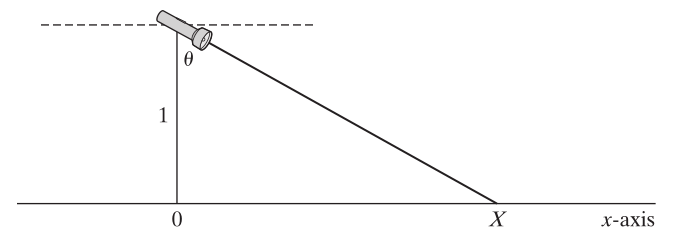
\includegraphics[scale=.6]{beam.PNG}
            \caption{Laser setup}
        \end{figure}

        \item Find the expectation $E[X]$.
    \end{enumerate}

    \item The time that it takes to service a car is an exponential random variable with rate 1.
    \begin{enumerate}
        \item If Alice brings her car in at time 0 and Bob brings in his car at time $t$, what is the probability that Bob's car is ready before Alice's? Assume that service times are independent and begin as soon as the car arrives.

        \item If both cars are brought in at time 0, with work starting on Bob's car only when Alice's car has been completely serviced, what is the probability that Bob's car is ready before time 2?
    \end{enumerate}

    \item If $X_1, X_2, \ldots, X_n$ are independent and identically distributed exponential random variables with parameter $\lambda$, compute
    \begin{enumerate}
        \item $\Pr[\min(X_1, \ldots, X_n) \leq a]$;
        \item $\Pr[\max(X_1, \ldots, X_n) \leq a]$;        
    \end{enumerate}

    \item The joint density function of $X$ and $Y$ is given by
    \[
        f(x,y) = c(x^2-y^2)e^{-x}\quad\text{if }x\geq 0,\ |y|\leq x.
    \]
    Find the conditional distribution of $Y$, given that $X = x$.

    \item Let $Z_1$ and $Z_2$ be independent standard normal random variables.
    Show that $X,Y$ has a bivariate normal distribution when $X = Z_1$ and $Y = Z_1+Z_2$.

    \item If $X$ and $Y$ are independent and identically distributed uniform random variables on $(0,1)$, compute the joint density of
    \begin{enumerate}
        \item $U = X+Y$, $V = X/Y$;
        \item $U = X+Y$, $V = X/(X+Y)$.
    \end{enumerate}

    \item Let $Z_1, Z_2, \ldots, Z_N$ be independent standard normal random variables and let
    \[
        S_n = \sum_{i=1}^n Z_i.
    \]
    \begin{enumerate}
        \item What is the conditional distribution of $S_n$ given that $S_k = y$, where $k$ is some integer between 1 and $n$?

        \item Show that for $1\leq k\leq n$, the conditional distribution of $S_k$ given that $S_n = x$ is normal with mean $xk/n$ and variance $k(n-k)/n$.
    \end{enumerate}


    \item Suppose $T_1, T_2, \ldots, T_n$ are continuous, independent, and identically distributed random variables.
    For any $k = 1, 2, \ldots, n$, find
    \[
        E\left(\frac{T_1 + T_2 + \cdots + T_k}{T_1 + T_2 + \cdots + T_n}\right).
    \]

    \item Suppose $G$ is a graph with $n$ vertices and $e$ edges.
    Show that you can partition the vertices of $G$ into two subsets $A$ and $B$ in such a way that at least half of the edges in $G$ cross between $A$ and $B$.

\end{enumerate}

\end{document}